\documentclass[UTF8, a4paper]{ctexart}
\usepackage{amssymb}
\usepackage{amsmath}
\usepackage{geometry}
\usepackage{graphicx}
\usepackage{float}
\usepackage{subfigure}
\usepackage{CJK}

\usepackage{lastpage}
\usepackage{titlesec}   %设置页眉页脚的宏包
\newpagestyle{main}{            
    \sethead{}{基于CP16的业余卫星通信系统}{page \thepage\ of \pageref{LastPage}}     %设置页眉
    %\setfoot{左页脚}{中页脚}{右页脚}      %设置页脚,可以在页脚添加 \thepage  显示页数
    \headrule                                      % 添加页眉的下划线
    \footrule                                       %添加页脚的下划线
}
\geometry{left=2cm, right=2cm, top=3cm, bottom=3cm}

\pagestyle{main}    %使用该style

  \author{无42 林子恒~2014011054\\
无42 刘若洋~2014011051\\
无42 王靖宇~2014011053\\
无48 黄志超~2013012062\\
无48 王~~~禹~2014011241}
  \title{基于CP16的业余卫星通信系统\\ \large{电子系统设计开题报告}}
  \date{}

\CTEXsetup[format={\Large\bfseries}]{section}

\begin{document}
    \maketitle
    \thispagestyle{empty}

  %% sections for contents
  \section{简介}
  业余卫星通讯,简称OSCAR (Orbiting Satellite Carrying Amateur Radio),是把绕行于地球轨道上的人造卫星,当作无线电通讯的中继器,以达到远程通讯的目的。在本项目中,我们将使用希望二号系列卫星,传输一段经由CP16编码过后的文字,经过卫星中继重新接收后,恢复出所发射的文字。
  
  \section{系统设计}
  \subsection{CP16编码系统}
  CP16是CRAC研发的汉字字形传输方式,抗干扰能力很强,适合于恶劣传输条件下的汉字报文通信。CP16可以被设想成是16路发射频率相近的CW信号,每路信号的开闭分别代表16×16汉字点阵的一列16个像素是否被点亮。这个信号在接收端显示屏的频谱-时间“瀑布图”上表现为一列亮点,随着时间的推移,依次显示出16行不同的列,组成一个完整的汉字图形,最终在接收机的频谱-时间瀑布图(简称瀑布图)上以“流水灯”的形式显示出报文。
分别使用 SDR Sharp 以及 Spectrum Lab 软件进行发射及收到信号频谱的展示,大致上效果应该会如下图所示:

   \begin{figure}[H]
%     \begin{minipage}[H]{1\linewidth}
       \centering
       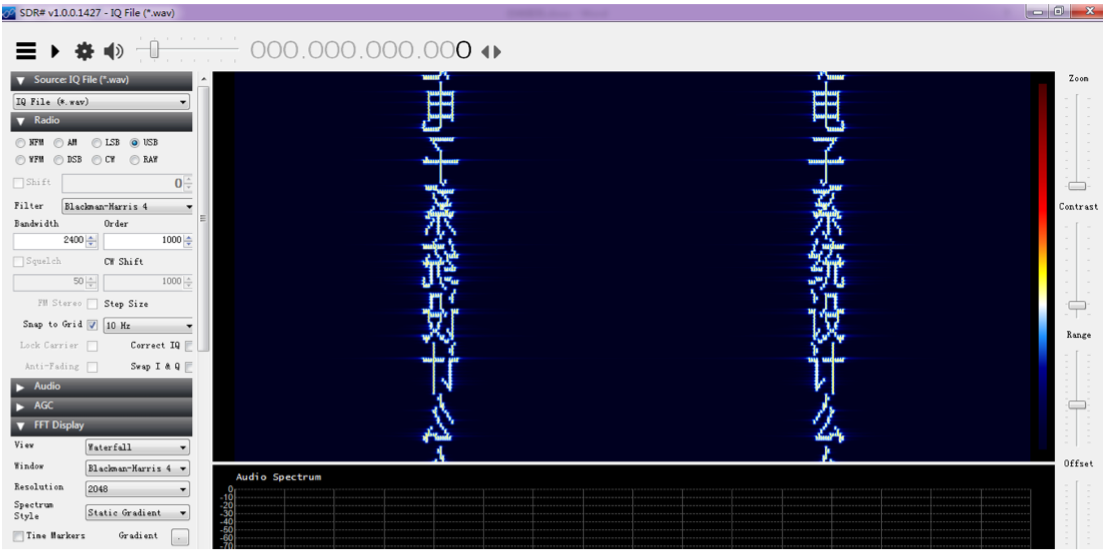
\includegraphics[width=9cm]{figure/sdr-sharp.png}
       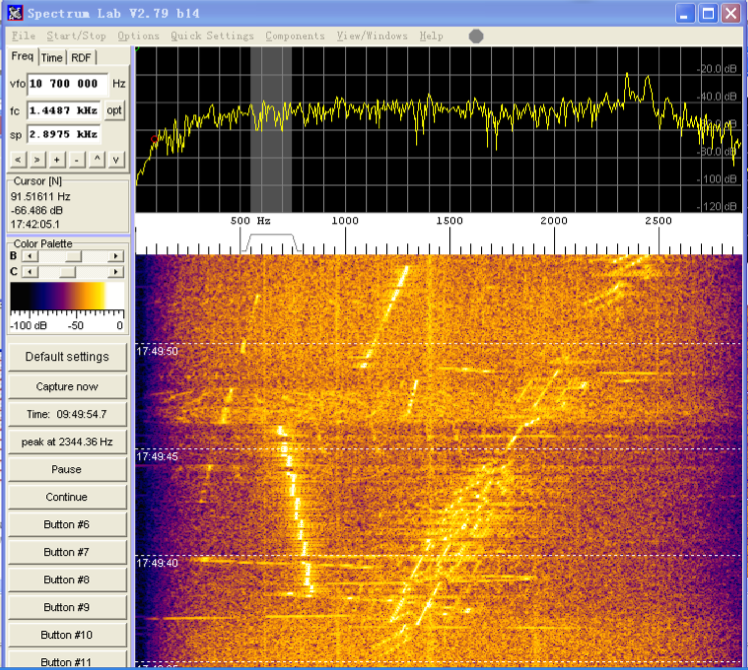
\includegraphics[width=5cm]{figure/spectrum-lab.png}
%     \end{minipage}
     \caption{SDR Sharp 以及 Spectrum Lab 软件展示}
   \end{figure}

  
  \subsection{收发信号}
  希望二号(XW-2)系列业余无线电卫星包括六颗卫星,命名为希望二A至希望二F。我们将使用g-predict软件确定卫星的轨迹和到来时间,并使用收发信机进行与卫星的通信,如下图所示:
     \begin{figure}[H]
     \begin{minipage}[H]{1\linewidth}
       \centering
       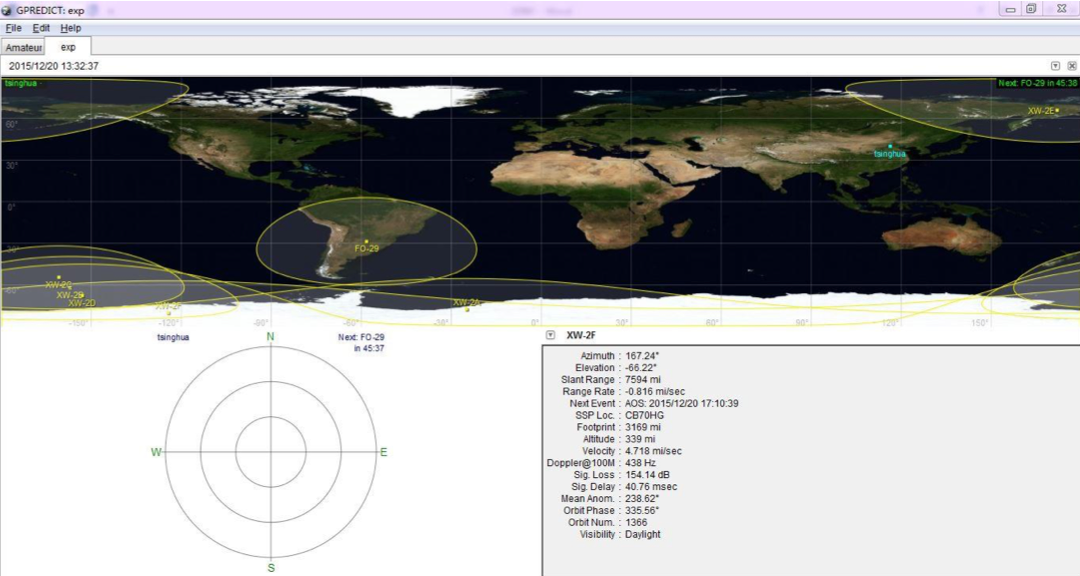
\includegraphics[width=10cm]{figure/gpredict.png}
       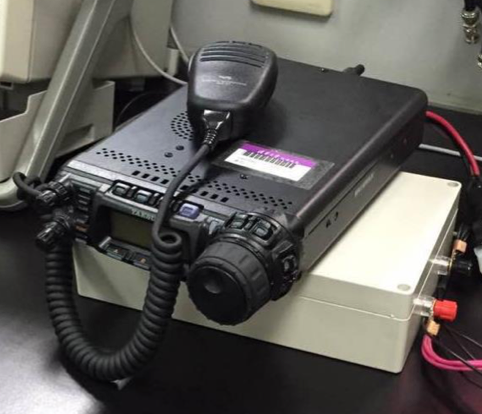
\includegraphics[width=6cm]{figure/trans-reciever.png}
     \end{minipage}
     \caption{g-predict软件 ~与~ 收发信机}
   \end{figure}
   
   
   %%
   \subsection{项目整体框架}
   \begin{enumerate}
   	\item 输入一串汉字之后,通过CP16编码系统,把汉字转换为一段音频
	\item 通过发射机将音频发送给卫星
	\item 通过收信机接收从卫星发射回来的信号
	\item 使用 Spectrum Lab 观察收到信号的瀑布图
  \end{enumerate}
   
      \begin{figure}[H]
%     \begin{minipage}[H]{1\linewidth}
       \centering
       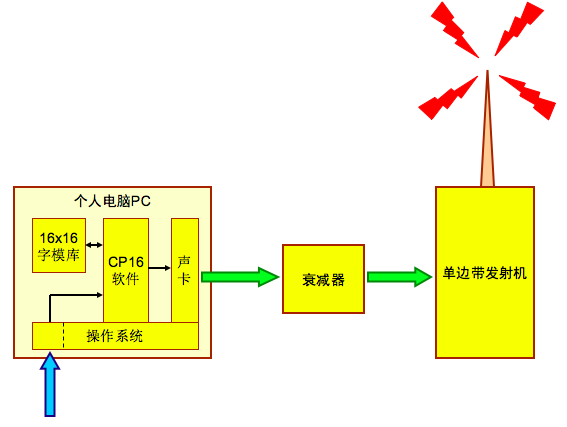
\includegraphics[width=7cm]{figure/system-trans.png}
       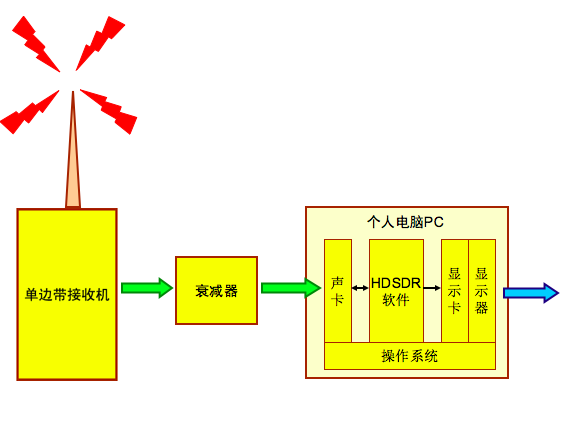
\includegraphics[width=7cm]{figure/system-rece.png}
%     \end{minipage}
     \caption{项目整体框架}
   \end{figure}
  
  \newpage
  \section{项目计划}
  \begin{enumerate}
    \item 调研并使用C++实现CP16算法
    \item 编写GUI,将CP16编码系统变得友好
    \item 学习g-predict软件以及收发机的操作及使用
    \item 调试系统,完成收发信号操作
    \item 解决多普勒效应的问题
    \item (选做)自做一个收信设备
  \end{enumerate}



  
  
\end{document}